% =====================================================================
%  Capítulo 2 — Estructura de un programa de defensa personal
% =====================================================================
\chapter{Estructura de un programa de defensa personal}

En la actualidad existen muchos sistemas de autoprotección, algunos con enfoque puramente técnico y otros con enfoque táctico. Encontraremos también sistemas que parten de enfoques específicos (policial, militar) que no son lo idóneo para la ciudadana común por las siguientes causas:

\begin{itemize}
  \item Quien creó el sistema y quien lo aprende no se enfrentan al mismo tipo de situaciones ni a agresores con los mismos objetivos.
  \item No suelen portar las mismas herramientas o armas.
  \item Tienen una predisposición y un entrenamiento psicológico muy distintos.
  \item Muchas técnicas van encaminadas a la contención, cuando lo que nos interesa es generar distancia para la interrupción y la huida.
  \item La legalidad para la que se pensó el sistema es diferente.
\end{itemize}

Esto no significa que no deban entrenarse esos sistemas, sino que deben considerarse ayudas para lograr la interrupción de la agresión y la huida.

Un sistema de autoprotección dirigido a civiles, asumiendo como objetivo la interrupción de la agresión y la huida del lugar, debería contener:

\begin{itemize}
  \item \textbf{Prevención y conciencia situacional} (el contenido más importante y el más rentable).
  \item \textbf{Habilidades verbales:} establecimiento de límites, desescalada, asertividad y uso de la voz.
  \item Bloqueos y cubiertas.
  \item Golpeos con armas corporales naturales (mano abierta, codo, rodilla, golpes bajos).
  \item Esquivas y desplazamientos.
  \item Agarres-sueltas y luxaciones simples.
  \item \textbf{Plan posterior:} huida, petición de ayuda, denuncia y autocuidado.
\end{itemize}

Todo ello trabajando desde distintas distancias: ambos de pie, pie-suelo, y ambos en el suelo.

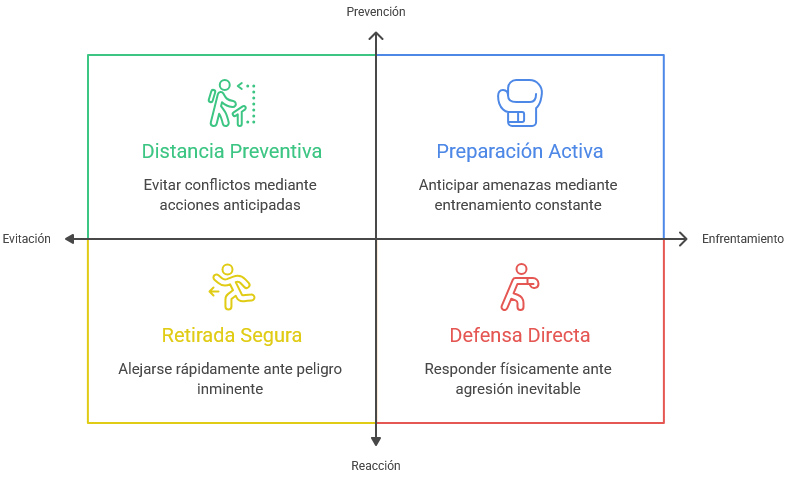
\includegraphics[width=\linewidth]{figures/evitacion.png}